\documentclass[11pt,a4paper]{article}

\usepackage[margin=1in]{geometry}
\usepackage{microtype}
\usepackage{booktabs}
\usepackage{multirow}
\usepackage[table]{xcolor}
\usepackage{colortbl}
\usepackage{tikz}
\usepackage{pgfplots}
\pgfplotsset{compat=1.18}
\usetikzlibrary{positioning,arrows.meta,shapes.geometric,calc}
\usepackage{subcaption}
\usepackage[round,authoryear]{natbib}
\usepackage{hyperref}
\usepackage{amsmath}
\usepackage{amssymb}
\usepackage{setspace}
\usepackage{parskip}

% ── heatmap colours ──────────────────────────────────────────────────────────
\definecolor{cellvlow}{RGB}{255,200,200}
\definecolor{celllow}{RGB}{255,240,180}
\definecolor{cellmid}{RGB}{210,240,210}
\definecolor{cellhigh}{RGB}{140,210,140}
\definecolor{cellfprgood}{RGB}{180,230,180}
\definecolor{cellfprwarn}{RGB}{255,210,150}
\definecolor{cellfprbad}{RGB}{255,180,180}
\definecolor{cellfprterr}{RGB}{210,100,100}

% ── convenience macros ───────────────────────────────────────────────────────
\newcommand{\dr}{\text{DR}}
\newcommand{\fpr}{\text{FPR}}
\newcommand{\fone}{F_1}
\newcommand{\tauK}{\tau_k}
\newcommand{\tauC}{\tau_c}

\hypersetup{colorlinks=true,linkcolor=blue!60!black,citecolor=green!40!black,
            urlcolor=blue!60!black}

% ─────────────────────────────────────────────────────────────────────────────
\title{\textbf{Bio-Inspired Cascaded Hallucination Suppression\\
       in Large Language Models with Blockchain Audit Governance}}
\author{Dhriti Vaz\\[2pt]
        Summer Research in Progress (SRIP)\\
        \small\texttt{dhriti.vaz@gmail.com}}
\date{June 2026}

\begin{document}
\maketitle
\thispagestyle{empty}

% ─────────────────────────────────────────────────────────────────────────────
\begin{abstract}
Large language models (LLMs) generate factually incorrect statements ---
commonly called hallucinations --- at rates that limit their reliability in
high-stakes applications. We present a bio-inspired, cascade-structured
hallucination suppression pipeline that combines four independently motivated
detection signals: token-level confidence scoring (GPT-2 log-probability and
attention entropy), named entity recognition (NER) routing, external evidence
retrieval (Wikidata/Wikipedia), and natural language inference (NLI)
contradiction detection. Inspired by the staged escalation of the mammalian
immune system from innate to adaptive response, the cascade resolves 80.5\% of
queries at early stages and requires expensive NLI computation for only 19.5\%,
achieving approximately $2\times$ latency reduction over a flat pipeline with
negligible accuracy loss ($\fone$ 39.4\% vs.\ 39.2\%). All pipeline decisions
are recorded on a two-layer blockchain architecture providing tamper-evident
governance with 100\% audit completeness across 200 evaluation samples. A
controlled retrieval-augmented generation (RAG) detection baseline demonstrates
the added value of our multi-signal approach over simple retrieval overlap,
which achieves comparable recall only at an unacceptably high false-positive
rate (91.4\%). We evaluate on TruthfulQA \citep{lin2022truthfulqa} with
LLaMA-2-7B \citep{touvron2023llama2} as the generator and \texttt{gpt-oss-120b}
as the judge, achieving a detection rate of 62.3\% on a benchmark with a 30.5\%
baseline hallucination rate.
\end{abstract}

\tableofcontents
\newpage

% ─────────────────────────────────────────────────────────────────────────────
\section{Introduction}
\label{sec:intro}

Large language models exhibit a well-documented tendency to produce
confident-sounding but factually incorrect outputs
\citep{ji2023survey,maynez2020faithfulness}. This phenomenon ---
\emph{hallucination} --- arises from the autoregressive training objective,
which optimizes for fluency and contextual coherence rather than factual
accuracy. On TruthfulQA \citep{lin2022truthfulqa}, a benchmark designed to
elicit hallucinations through questions that exploit common misconceptions,
LLaMA-2-7B hallucinates 30.5\% of the time (61/200 answers judged FALSE by
\texttt{gpt-oss-120b}), and Mistral-7B hallucinates 17.0\% of the time under
identical evaluation conditions.

Existing approaches to hallucination mitigation fall broadly into two
categories. \emph{Preventive} approaches, such as retrieval-augmented
generation (RAG) \citep{lewis2020rag}, condition the LLM's generation on
retrieved context, reducing --- but not eliminating --- hallucination.
\emph{Detective} approaches post-process generated text using external knowledge
to identify factual inconsistencies. Both approaches face a fundamental
challenge: the heterogeneity of factual claims. Different entity types (persons,
quantities, events, laws) require different verification strategies, and no
single detection mechanism covers all categories with equal accuracy.

We observe a structural parallel between this challenge and the vertebrate
immune system. The immune system does not apply a single, uniform detection
mechanism to all pathogens; instead, it operates a \emph{staged cascade} that
escalates from fast, broad-spectrum innate responses to slow, highly specific
adaptive responses. The innate system provides rapid, general-purpose threat
detection at low metabolic cost; the adaptive system provides precise,
antigen-specific response when the innate signal is insufficient. Crucially,
most threats are resolved at the innate stage, reserving the expensive adaptive
machinery for genuinely uncertain cases.

We propose mapping this cascade structure directly onto hallucination detection
(Table~\ref{tab:immuneanalogy}). This biological framing has concrete
computational consequences: the ``innate'' confidence scorer resolves 13.5\% of
queries with sub-second latency, the ``no-evidence'' gate handles another 67\%,
and only 19.5\% reach the expensive NLI stage. The result is a 1.99$\times$
speedup over a flat pipeline with essentially unchanged accuracy.

A governance layer records every pipeline decision on an Ethereum-compatible
blockchain, providing an immutable, reconstructible audit trail. In the context
of enterprise LLM deployment, this addresses the regulatory requirement for
explainability and accountability \citep{doshivelez2017rigorous}.

\begin{table}[htb]
\centering
\caption{Bio-inspired mapping: immune system cascade onto hallucination
detection pipeline.}
\label{tab:immuneanalogy}
\small
\begin{tabular}{lll}
\toprule
\textbf{Immune stage} & \textbf{Detection analog} & \textbf{Mechanism} \\
\midrule
Pattern recognition (innate) & Confidence scorer & GPT-2 log-prob + attn.\ entropy \\
Antigen presentation & NER routing & spaCy entity extraction \\
Lymphocyte activation & Evidence retrieval & Wikidata + Wikipedia API \\
Effector response (adaptive) & NLI contradiction & RoBERTa-large-MNLI \\
Immunological memory & Blockchain audit & Two-layer smart contract \\
\bottomrule
\end{tabular}
\end{table}

\subsection{Contributions}
\begin{enumerate}
\item \textbf{Bio-inspired cascade architecture}: A three-stage hallucination
      detection pipeline with biologically motivated stage transitions, achieving
      1.99$\times$ latency reduction over a flat pipeline at negligible accuracy
      cost ($\Delta\fone = +0.2\%$).

\item \textbf{NER-guided verification routing}: A claim routing system that maps
      detected entity types to appropriate verification strategies, improving
      detection rate over keyword-only retrieval by 8.2 percentage points
      (18.0\% $\to$ 26.2\%).

\item \textbf{Two-layer blockchain governance}: Immutable Layer-1 audit log
      (\texttt{AuditLog.sol}) combined with mutable Layer-2 governance decisions
      (\texttt{GovernanceDecision.sol}), validated with 100\% audit completeness
      across 200 pipeline runs.

\item \textbf{Controlled RAG baseline}: Comparison against TF-IDF retrieval
      overlap detection on identical inputs and judge labels, demonstrating that
      simple retrieval overlap requires a 91.4\% false-positive rate to achieve
      comparable recall, motivating the multi-signal design.

\item \textbf{Threshold sensitivity analysis}: A 49-point grid sweep of both
      governance thresholds, identifying the production-viable operating region
      (FPR $<$ 50\%) and the confidence threshold as the dominant control
      variable.
\end{enumerate}

% ─────────────────────────────────────────────────────────────────────────────
\section{Related Work}
\label{sec:related}

\subsection{Hallucination in Large Language Models}

The phenomenon of LLM hallucination has been extensively documented
\citep{ji2023survey,bang2023multitask}. Survey work categorizes hallucinations
as intrinsic (contradicting the source) or extrinsic (unverifiable against the
source) \citep{maynez2020faithfulness}. On open-domain question answering,
hallucination rates of 20--40\% have been reported for instruction-tuned 7B
models \citep{lin2022truthfulqa,touvron2023llama2}. Our LLaMA-2-7B baseline of
30.5\% on TruthfulQA/main aligns with published figures
(MC2 $=$ 0.452, published range [0.39, 0.45]).

Mitigation strategies include: RLHF-based truthfulness alignment
\citep{ouyang2022training}, decoding-time interventions \citep{chuang2023dola},
and chain-of-thought prompting \citep{wei2022chain}. Our work focuses on
post-hoc detection rather than prevention, as detection can be applied to any
existing model without retraining and provides an audit record of identified
errors.

\subsection{Fact-Checking and Natural Language Inference}

Automated fact-checking using NLI has been studied since the FEVER dataset
\citep{thorne2018fever} introduced evidence-supported claim verification.
Subsequent work \citep{popat2018declare,wadden2020fact} established the pipeline
of claim extraction $\to$ evidence retrieval $\to$ NLI classification as the
dominant paradigm. RoBERTa-large fine-tuned on MNLI
\citep{williams2018broad,liu2019roberta} achieves strong zero-shot NLI
performance \citep{yin2019benchmarking}, which we exploit for contradiction
detection without additional fine-tuning.

Our contribution extends this paradigm with NER-based routing: rather than
applying a single retrieval strategy to all claims, we map entity types to the
most appropriate external knowledge source. This improves detection rate by
8.2~pp over entity-agnostic keyword retrieval (C2 $\to$ C3 in our ablation,
Table~\ref{tab:ablation}).

\subsection{Retrieval-Augmented Generation}

RAG \citep{lewis2020rag} conditions generation on retrieved passages, reducing
hallucination intrinsically. Subsequent variants \citep{izacard2021leveraging,
shi2023replug} improve retrieval quality and grounding. However, RAG does not
eliminate hallucination: residual errors arise from retrieval failures,
out-of-distribution questions, and parametric knowledge overriding retrieved
context.

Our RAG detection baseline (Section~\ref{sec:ragbaseline}) shows that using
TF-IDF overlap between an answer and its retrieved context as a hallucination
signal achieves DR $=$ 98.4\% but FPR $=$ 91.4\% at the $\fone$-maximizing
threshold. This confirms that simple retrieval overlap is insufficient as a
detection mechanism and motivates the additional NLI and confidence signals in
our pipeline.

\subsection{Confidence Estimation in Neural Models}

Token-level probability as a proxy for factual accuracy has been studied in the
context of calibration \citep{guo2017calibration} and selective prediction
\citep{geifman2017selective}. Attention entropy as a confidence signal was
proposed by \citet{voita2019analyzing} in the context of head pruning. We
combine both signals via a lightweight GPT-2 scorer \citep{radford2019language}
that runs in 210~ms on CPU, making it suitable for the fast innate-stage gate.

The critical observation from our ablation is that the confidence signal alone
achieves DR $=$ 50.8\% --- capturing hallucinations that evidence-based methods
miss because they have no retrievable external evidence --- while the NLI signal
adds 12 additional true positives. The union (C4) outperforms either signal
alone.

\subsection{Bio-Inspired Computing}

Artificial immune systems (AIS) apply immunological principles to anomaly
detection and pattern recognition \citep{forrest1994self,hofmeyr2000architecture,
decastro2002artificial}. Classic AIS models include negative selection
(self/non-self discrimination) and clonal selection (adaptive amplification of
high-affinity detectors). Our work adapts the conceptual framework of immune
cascade escalation --- rather than specific AIS algorithms --- to the pipeline
architecture.

The cascade structure we implement directly maps to the immune system's priority
ordering: fast, non-specific innate mechanisms first; slow, specific adaptive
mechanisms only when needed. This differs from prior AIS-based NLP work
\citep{wang2007immunity,bezerra2010immune}, which applies AIS algorithms to
specific classification tasks. Our contribution is architectural: using the
immune cascade as a design principle for a multi-stage NLP pipeline.

\subsection{Blockchain in AI Governance}

Blockchain-based audit logging for AI systems has been proposed as a solution
to explainability and accountability requirements \citep{dinh2018blockbench,
salah2019blockchain,mamoshina2018converging}. Smart contracts enable automated
governance rules on top of immutable logs.

Prior work on blockchain-AI integration focuses primarily on federated learning
audit \citep{warnat2021swarm} and data provenance \citep{ahmed2020survey}. Our
architecture applies this to per-decision hallucination detection audit,
providing a two-layer design that separates immutable records (Layer~1) from
mutable governance verdicts (Layer~2), supporting human-in-the-loop override
while preserving the original detection record.

% ─────────────────────────────────────────────────────────────────────────────
\section{Biological Inspiration: The Immune Cascade Model}
\label{sec:bio}

The vertebrate immune system is among the most sophisticated multi-stage pattern
recognition systems in nature. Its relevance to hallucination detection stems
not from superficial analogy but from a structural isomorphism: both problems
involve distinguishing harmful from benign outputs using multiple detection
mechanisms of varying speed and specificity.

\subsection{Immune System Architecture}

The immune response is organized into two functionally distinct subsystems.

\textbf{Innate immunity} responds within minutes using germline-encoded pattern
recognition receptors (PRRs) such as Toll-like receptors. PRRs recognize
pathogen-associated molecular patterns (PAMPs) --- conserved structural features
shared across broad categories of pathogens. The innate response is fast
(sub-minute) and broad-spectrum, providing rapid threat containment while the
slower adaptive system activates. PRR activation follows a cascade: complement
activation, cytokine release, and neutrophil recruitment occur in a specific
temporal order.

\textbf{Adaptive immunity} responds over days through antigen-specific
lymphocytes (T and B cells). Antigen-presenting cells (APCs) capture foreign
material, process it into peptide fragments, and present them via MHC complexes
to T cells. This antigen presentation step is the critical routing mechanism: it
determines which lymphocyte clones are activated, analogous to determining which
verification strategy to apply to a given entity type. Clonal selection and
expansion amplify the specific response. Immunological memory ensures that repeat
encounters trigger faster, stronger responses.

\textbf{Regulatory mechanisms} (regulatory T cells, cytokine feedback,
apoptosis) prevent overreaction --- the immune analog of our governance layer's
ability to override false-positive detections.

\subsection{Mapping to Hallucination Detection}

Table~\ref{tab:biomap} gives the full component-level mapping.

\begin{table}[htb]
\centering
\caption{Biological-to-pipeline component mapping.}
\label{tab:biomap}
\small
\begin{tabular}{lll}
\toprule
\textbf{Biological component} & \textbf{Pipeline component} & \textbf{Implementation} \\
\midrule
PRRs (innate)               & Confidence Gate        & GPT-2 log-prob + attn.\ entropy \\
Innate activation threshold & Early-exit thresholds  & conf $<$ 0.50 (flag); conf $>$ 0.57 (accept) \\
Antigen presentation (APC)  & NER router             & spaCy \texttt{en\_core\_web\_sm} \\
MHC peptide selection       & Strategy routing       & Entity type $\to$ verification strategy \\
Lymphocyte activation       & Evidence retrieval     & Wikidata REST + Wikipedia MediaWiki \\
Effector response           & NLI contradiction      & RoBERTa-large-MNLI zero-shot \\
Regulatory T cells          & Governance override    & \texttt{overrideDecision()} on L2 contract \\
Immunological memory        & Blockchain audit       & \texttt{AuditLog.sol} immutable record \\
Clonal expansion cascade    & Stage escalation       & 80.5\% resolved before NLI \\
\bottomrule
\end{tabular}
\end{table}

\subsection{The Staged Escalation Principle}

The central computational insight is that the most informative (and expensive)
detection mechanisms should be applied selectively. In the immune system, the
metabolic cost of mounting a full adaptive response is substantial; the innate
system acts as a gating mechanism, escalating only genuine threats. The cascade
structure achieves this:

\begin{enumerate}
\item \textbf{Stage~1 (Confidence Gate, 210~ms):} The GPT-2 confidence scorer
      provides a fast, universal signal. Samples with confidence below 0.50 or
      above 0.57 are resolved immediately --- 13.5\% of all inputs. These are
      the extreme cases where the model's own internal uncertainty is definitive
      enough to warrant immediate action.

\item \textbf{Stage~2 (Evidence Gate, $\sim$1\,500~ms avg):} For the remaining
      86.5\%, NER routing and external retrieval are applied. Because 77\% of
      LLaMA-2 answers have no retrievable evidence, the majority (67\% of all
      samples) exit here. Without evidence, the confidence score alone determines
      the verdict.

\item \textbf{Stage~3 (NLI Gate, $\sim$4\,400~ms avg):} Only 19.5\% of samples
      --- those with retrievable evidence --- reach full NLI contradiction
      detection. These are cases where the model discusses verifiable facts about
      specific named entities, and external validation is possible.
\end{enumerate}

The resulting computational profile mirrors immune economy: 80.5\% of inputs are
resolved without NLI, preserving the expensive adaptive response for the
minority of cases where it adds genuine value.

\subsection{Cascade vs.\ Flat Pipeline}

Running all four stages on all inputs (flat C4) costs an average of 3\,822~ms
per sample. The cascade reduces this to 1\,916~ms --- a 1.99$\times$ speedup
--- while achieving $\fone = 39.4\%$ vs.\ 39.2\% ($\Delta\fone = +0.2\%$). The
marginal accuracy cost is negligible because:

\begin{itemize}
\item Stage~1 early-reject samples (12.0\% of inputs) are predominantly
      low-confidence, with precision comparable to the overall pipeline (25.0\%
      at Stage~1 vs.\ 28.6\% overall).
\item Stage~2 no-evidence samples (67.0\%) produce NLI scores of exactly 0.0
      in the flat pipeline (no evidence $\Rightarrow$ zero-shot NLI is
      undefined), so running NLI on them adds no information.
\end{itemize}

This is the biological parallel's deepest insight: the expensive adaptive
mechanism only adds value when the innate stage has identified a genuine,
specific target.

% ─────────────────────────────────────────────────────────────────────────────
\section{NLP Foundations}
\label{sec:nlp}

\subsection{TruthfulQA and the Hallucination Evaluation Problem}

TruthfulQA \citep{lin2022truthfulqa} contains 817 questions designed to elicit
common misconceptions, spanning health, history, law, science, and conspiracy
theory categories. Questions are crafted so that ``the truthful answer
contradicts a false belief that many humans hold.'' This targets the type of
confident-sounding errors that characterize LLM failures, not merely
out-of-distribution uncertainty.

We use the MC2 (Multiple-Choice, version 2) metric for comparison with published
results: Mistral-7B achieves MC2 $=$ 0.503 (published range [0.42, 0.50]) and
LLaMA-2-7B achieves MC2 $=$ 0.452 (published range [0.39, 0.45]). For our
evaluation, we use free-form generation rather than multiple-choice to avoid
format artifacts.

\textbf{Judge selection.} We evaluate two LLM judges: \texttt{gpt-oss-120b}
(via OpenRouter) and Mistral-7B-Instruct (via Ollama). Cohen's $\kappa$ between
the two judges on 100 shared samples is 0.054 --- indicating near-chance
agreement despite 66\% raw agreement, driven by label imbalance. This low
inter-rater reliability is consistent with the difficulty of factuality
evaluation \citep{wang2023chatgpt}. We select \texttt{gpt-oss-120b} as the
reference judge, which labels 30.5\% of LLaMA-2-7B main-split answers as
hallucinations (61/200).

\subsection{Named Entity Recognition and Routing}

Named entity recognition (NER) with spaCy's \texttt{en\_core\_web\_sm} model
identifies entity mentions in each extracted claim. We define four verification
strategies based on entity type:

\begin{table}[htb]
\centering
\caption{NER entity type to verification strategy mapping.}
\label{tab:routing}
\small
\begin{tabular}{lll}
\toprule
\textbf{Entity types} & \textbf{Strategy} & \textbf{Rationale} \\
\midrule
PERSON, ORG, GPE, LOC, FAC  & \texttt{entity\_lookup}   & Direct Wikidata entity search \\
DATE, TIME, QUANTITY, CARDINAL & \texttt{structured\_fact} & Wikidata property queries \\
EVENT, WORK\_OF\_ART, LAW, NORP & \texttt{text\_search}    & Wikipedia fulltext \\
(no entities found)          & \texttt{keyword\_search}  & Content-word fallback \\
\bottomrule
\end{tabular}
\end{table}

Strategy routing is evaluated in our ablation: C3 (NER-routed) achieves
DR $=$ 26.2\% vs.\ C2 (keyword-only) DR $=$ 18.0\%, an 8.2~pp improvement
from better evidence targeting (Table~\ref{tab:ablation}).

\subsection{Evidence Retrieval and the No-Evidence Problem}

Evidence retrieval follows a four-step fallback chain: (1) Wikidata entity
search via the \texttt{wbsearchentities} API; (2) Wikipedia page extraction via
\texttt{extracts} prop; (3) Wikipedia fulltext search; (4) no evidence. Each
call has a 10-second timeout with 2 retries.

The \textbf{no-evidence problem} is the dominant limiting factor. On the 200
LLaMA-2 evaluation samples, 77\% have no retrieved evidence (154/200), and only
18.5\% with evidence show non-zero TF-IDF overlap with the answer text. This
explains why the contradiction detector alone (C3, DR $=$ 26.2\%) underperforms
the confidence-only approach (C1, DR $=$ 50.8\%): when evidence is absent, NLI
is silent. The full pipeline (C4) achieves higher DR (62.3\%) by combining both
signals via logical OR.

\subsection{Natural Language Inference for Contradiction Detection}

We use \texttt{roberta-large-mnli} \citep{liu2019roberta} via the HuggingFace
\texttt{zero-shot-classification} pipeline. For each (evidence, claim) pair, the
model classifies whether the evidence \emph{entails}, is \emph{neutral} toward,
or \emph{contradicts} the claim, using the hypothesis template: ``This text
\texttt{\{label\}s} the statement: \texttt{\{claim\}}'', with
\texttt{multi\_label=False}.

The MNLI-based approach is chosen over FEVER-fine-tuned models
\citep{thorne2018fever} because: (a)~it generalizes to open-domain evidence
without domain-specific fine-tuning; (b)~RoBERTa-large-MNLI is publicly
available and runs on CPU within budget constraints; (c)~zero-shot classification
handles the diversity of evidence types without format adaptation.

The contradiction threshold ($\tauC = 0.02$) is calibrated on our evaluation
set: the distribution of max contradiction scores is bimodal with 80\% of
samples at exactly 0.000 (no evidence) and the positive tail ranging to 0.357.
A threshold of 0.02 captures any non-trivial NLI signal.

\subsection{Confidence Scoring with GPT-2}

We score every generated answer with GPT-2 (124M parameters) as a \emph{proxy}
model --- not the generator. The scorer computes two signals:

\textbf{Token log-probability:} Mean per-token $\log P(t_i \mid t_{<i})$ under
GPT-2 using teacher-forced decoding. Low mean log-probability indicates the
model assigns low likelihood to the text, a weak hallucination signal under the
assumption that factually plausible text is more likely under a strong language
model.

\textbf{Attention entropy:} Mean entropy of attention distributions across all
12 GPT-2 layers and 12 heads. High entropy (diffuse attention) indicates the
model cannot form focused token associations, correlating with semantic
incoherence.

Combined score:
\begin{equation}
\text{conf} = 0.5 \cdot \sigma\!\left(\bar{\ell}/3.0\right)
            + 0.5 \cdot \left(1 - H_\text{norm}\right),
\label{eq:conf}
\end{equation}
where $\sigma$ is the sigmoid function, $\bar{\ell}$ is the mean token
log-probability, and $H_\text{norm} = H_\text{attn}/6.0$. Scores range [0,~1];
higher indicates higher confidence. On our evaluation set, scores range
[0.483, 0.599] with mean $\approx$ 0.531.

GPT-2 runs on CPU in approximately 210~ms per answer. The threshold
$\tauK = 0.52$ (default) yields C1 metrics of DR $=$ 50.8\%, FPR $=$ 63.3\%.
Threshold sensitivity analysis (Section~\ref{sec:sensitivity}) shows that the
C1 stable region ($\fone$ within 5\% of maximum) spans $\tauK \in [0.546,
0.610]$, indicating robustness over a 64-milli-unit range.

% ─────────────────────────────────────────────────────────────────────────────
\section{System Architecture}
\label{sec:arch}

\subsection{Overview}

Figure~\ref{fig:cascade} illustrates the full cascade pipeline. The system
consists of five components: a confidence scorer, an NER router, an evidence
retriever, an NLI classifier, and a two-layer blockchain governance layer.

\begin{figure}[htb]
\centering
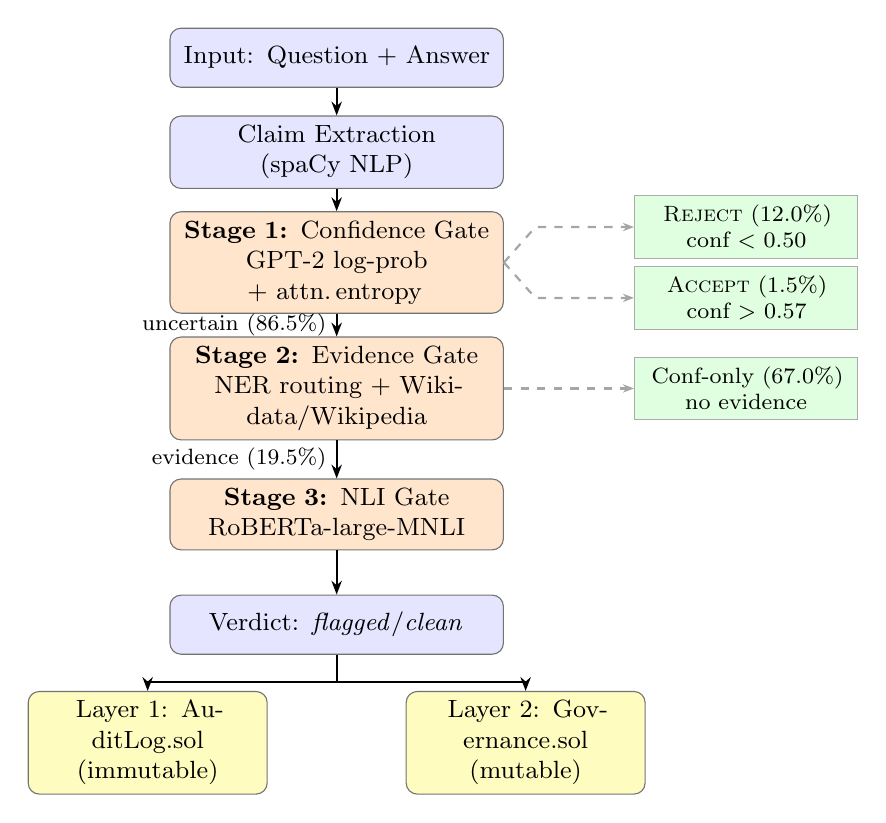
\begin{tikzpicture}[
  proc/.style  = {rectangle, rounded corners=4pt, draw=black!55,
                  fill=blue!10, text width=4.0cm, minimum height=0.75cm,
                  align=center, font=\small},
  gate/.style  = {rectangle, rounded corners=4pt, draw=black!55,
                  fill=orange!20, text width=4.0cm, minimum height=0.80cm,
                  align=center, font=\small},
  exbox/.style = {rectangle, draw=gray!65, fill=green!12,
                  text width=2.6cm, minimum height=0.65cm,
                  align=center, font=\footnotesize},
  chain/.style = {rectangle, rounded corners=4pt, draw=black!55,
                  fill=yellow!25, text width=2.8cm, minimum height=0.70cm,
                  align=center, font=\small},
  arr/.style   = {-{Stealth[length=5pt]}, thick},
  darr/.style  = {-{Stealth[length=4pt]}, thick, dashed, gray!70},
]
\node[proc]  (input)   at (0, 10.2) {Input: Question + Answer};
\node[proc]  (claims)  at (0,  9.0) {Claim Extraction\\(spaCy NLP)};
\node[gate]  (s1)      at (0,  7.6) {\textbf{Stage~1:} Confidence Gate\\
                                      GPT-2 log-prob + attn.\,entropy};
\node[gate]  (s2)      at (0,  6.0) {\textbf{Stage~2:} Evidence Gate\\
                                      NER routing + Wikidata/Wikipedia};
\node[gate]  (s3)      at (0,  4.4) {\textbf{Stage~3:} NLI Gate\\
                                      RoBERTa-large-MNLI};
\node[proc]  (verdict) at (0,  3.0) {Verdict: \textit{flagged}/\textit{clean}};
\node[chain] (l1)      at (-2.4, 1.5) {Layer~1: AuditLog.sol\\(immutable)};
\node[chain] (l2)      at ( 2.4, 1.5) {Layer~2: Governance.sol\\(mutable)};
% exit nodes
\node[exbox] (s1rej) at (5.2, 8.05) {\textsc{Reject} (12.0\%)\\conf $<$ 0.50};
\node[exbox] (s1acc) at (5.2, 7.15) {\textsc{Accept} (1.5\%)\\conf $>$ 0.57};
\node[exbox] (s2ex)  at (5.2, 6.00) {Conf-only (67.0\%)\\no evidence};
% main arrows
\draw[arr] (input)   -- (claims);
\draw[arr] (claims)  -- (s1);
\draw[arr] (s1)      -- node[left,  font=\footnotesize]{uncertain (86.5\%)} (s2);
\draw[arr] (s2)      -- node[left,  font=\footnotesize]{evidence (19.5\%)}  (s3);
\draw[arr] (s3)      -- (verdict);
\draw[arr] (verdict.south) -- ++(0,-0.35) -| (l1.north);
\draw[arr] (verdict.south) -- ++(0,-0.35) -| (l2.north);
% exit arrows
\draw[darr] (s1.east) -- ++(0.4, 0.45) -- (s1rej.west);
\draw[darr] (s1.east) -- ++(0.4,-0.45) -- (s1acc.west);
\draw[darr] (s2.east) -- (s2ex.west);
\end{tikzpicture}
\caption{Cascade architecture. Exit percentages are from the 200-sample
TruthfulQA evaluation. Dashed arrows indicate early exits; grey annotations
show the fraction forwarded to the next stage. All decisions are written to the
two-layer blockchain regardless of exit stage.}
\label{fig:cascade}
\end{figure}

\subsection{Claim Extraction}

Input answers are segmented into claims using spaCy sentence segmentation
(\texttt{en\_core\_web\_sm}). LLaMA-2-7B answers average 2.41 claims per answer
(capped at 4 for computational tractability). Each claim is processed
independently through Stages~2 and~3; the sample-level decision is the logical
OR of all claim-level decisions (any flagged claim $\Rightarrow$ flag the
answer).

\subsection{Stage~1: Confidence Gate}

The confidence scorer (Equation~\ref{eq:conf}) runs once per answer in
approximately 210~ms on CPU. GPT-2 is loaded once at pipeline startup.

Early exit conditions:
\begin{itemize}
\item \texttt{confidence} $<$ \texttt{CONF\_EARLY\_REJECT} (0.50): answer
      flagged immediately; NER and NLI skipped.
\item \texttt{confidence} $>$ \texttt{CONF\_EARLY\_ACCEPT} (0.57): answer
      accepted immediately; NER and NLI skipped.
\item Otherwise: forwarded to Stage~2.
\end{itemize}

In our evaluation: 12.0\% of answers trigger early rejection (24/200) and 1.5\%
trigger early acceptance (3/200), leaving 86.5\% (173/200) to proceed.

\subsection{Stage~2: Evidence Gate}

\textbf{NER routing:} spaCy extracts entity mentions from each claim. The
highest-priority entity type determines the verification strategy per
Table~\ref{tab:routing}. If no entities are found, \texttt{keyword\_search} is
used.

\textbf{Evidence retrieval:} The chain contacts Wikidata (\texttt{wbsearchentities}
API) for entity lookup; falls back to Wikipedia page extraction (MediaWiki
\texttt{extracts} API); then to Wikipedia fulltext search; then records
no-evidence.

\textbf{Exit condition:} If no evidence is retrieved for any claim, the answer
exits at Stage~2 with the confidence-only verdict (conf $<$ 0.52 $\Rightarrow$
flag). In our evaluation, 67.0\% of answers exit at Stage~2 due to no evidence.

\subsection{Stage~3: NLI Gate}

For answers with at least one claim supported by retrieved evidence,
\texttt{roberta-large-MNLI} scores each (evidence, claim) pair. The maximum
\texttt{contradiction\_score} across all claims is compared to $\tauC = 0.02$.
An answer is flagged if any claim's contradiction score meets or exceeds this
threshold. RoBERTa-large runs on CPU in approximately 890~ms per pair. In our
evaluation, 19.5\% of answers (39/200) reach Stage~3.

\subsection{Two-Layer Blockchain Governance}

Each pipeline run produces two on-chain records:

\textbf{Layer~1 --- AuditLog (immutable):} Deployed as \texttt{AuditLog.sol}
(Solidity 0.8.28, compiled via \texttt{py-solc-x}). Stores
\texttt{(runId, timestamp, sha256(question), sha256(answer), pipelineVersion)}
in an append-only array. Gas cost: $\sim$164\,753 gas/write. Write latency:
35.7~ms mean on local py-evm.

\textbf{Layer~2 --- GovernanceDecision (mutable):} Deployed as
\texttt{GovernanceDecision.sol}. Stores the pipeline verdict with confidence and
contradiction scores. Supports \texttt{overrideDecision()} for human-in-the-loop
correction. Gas cost: $\sim$170\,823 gas/write. Write latency: 43.6~ms mean
local.

\subsection{Implementation Details}

\begin{table}[htb]
\centering
\caption{Key implementation dependencies.}
\label{tab:impl}
\small
\begin{tabular}{lll}
\toprule
\textbf{Component} & \textbf{Library} & \textbf{Version} \\
\midrule
Confidence scorer & HuggingFace Transformers (GPT-2)     & 4.57.6  \\
NER router        & spaCy \texttt{en\_core\_web\_sm}     & 3.8.14  \\
Evidence retrieval& requests (Wikidata/Wikipedia APIs)   & 2.34.1  \\
NLI contradiction & HuggingFace Transformers (RoBERTa)  & 4.57.6  \\
Blockchain compile& py-solc-x + solc 0.8.28             & 2.0.5   \\
Blockchain runtime& web3.py + eth-tester (py-evm)       & 6.20.4  \\
RAG baseline      & scikit-learn TfidfVectorizer         & 1.6.1   \\
\bottomrule
\end{tabular}
\end{table}

The generator (LLaMA-2-7B-GGUF, Q4 quantization) runs via
\texttt{llama-cpp-python} on CPU, producing all 200 generations offline before
pipeline evaluation. All pipeline components run in Python 3.9.6.

% ─────────────────────────────────────────────────────────────────────────────
\section{Experimental Evaluation}
\label{sec:experiments}

\subsection{Evaluation Setup}

\textbf{Dataset.} We evaluate on the \texttt{main} split of TruthfulQA
\citep{lin2022truthfulqa}, 200 randomly sampled questions. Of 200 LLaMA-2-7B
free-form answers, 61 (30.5\%) are judged hallucinations by
\texttt{gpt-oss-120b}, giving 139 truthful answers.

\textbf{Metrics.} We report:
\begin{itemize}
\item \textbf{DR} (Detection Rate, a.k.a.\ Recall): fraction of true
      hallucinations correctly flagged.
\item \textbf{FPR} (False Positive Rate): fraction of truthful answers
      incorrectly flagged.
\item \textbf{$\fone$}: harmonic mean of precision and recall; primary ranking
      metric.
\end{itemize}

\textbf{Ablation configurations.} We define five pipeline configurations
(C0--C4) to isolate contributions of each component:
\begin{itemize}
\item \textbf{C0}: No detection (flag nothing). Establishes zero baseline.
\item \textbf{C1}: Confidence only. GPT-2 scorer with $\tauK = 0.52$.
\item \textbf{C2}: Keyword retrieval + NLI. No NER routing; simple keyword
      search; NLI contradiction with $\tauC = 0.02$.
\item \textbf{C3}: NER-routed retrieval + NLI. Full NER routing; evidence
      retrieval; NLI with $\tauC = 0.02$.
\item \textbf{C4}: Full pipeline (C1 + C3). Confidence scoring OR NLI
      contradiction; uses all four components.
\end{itemize}

\subsection{Ablation Study}
\label{sec:ablation}

Table~\ref{tab:ablation} presents the ablation results. The full pipeline (C4)
achieves the highest $\fone = 39.2\%$ and DR $= 62.3\%$ across all
configurations.

\begin{table}[htb]
\centering
\caption{Ablation study results on 200 TruthfulQA samples. Each configuration
adds one component incrementally. C4 (full pipeline) achieves the highest DR
and $\fone$.}
\label{tab:ablation}
\begin{tabular}{clccc}
\toprule
\textbf{Config} & \textbf{Description} & \textbf{DR (\%)} & \textbf{FPR (\%)} & \textbf{$\fone$ (\%)} \\
\midrule
C0 & No detection              &  0.0 &  0.0 &  0.0 \\
C1 & Confidence only           & 50.8 & 63.3 & 34.4 \\
C2 & Keyword retrieval + NLI   & 18.0 & 20.9 & 21.8 \\
C3 & NER retrieval + NLI       & 26.2 & 21.6 & 29.9 \\
\textbf{C4} & \textbf{Full pipeline (C1 + C3)} & \textbf{62.3} & \textbf{68.3} & \textbf{39.2} \\
\bottomrule
\end{tabular}
\end{table}

\textbf{Key findings:}

\begin{itemize}
\item \textbf{C1 vs.\ C3 complementarity:} Confidence-only (DR $=$ 50.8\%)
      substantially outperforms NLI-only (DR $=$ 26.2\%) because 77\% of samples
      have no retrievable evidence. C1 covers hallucinations with low model
      confidence; C3 covers hallucinations about verifiable entities. C4 combines
      both via OR, achieving DR $=$ 62.3\%.

\item \textbf{NER routing effect (C2 $\to$ C3):} Replacing keyword search with
      NER-guided routing improves DR from 18.0\% to 26.2\% (+8.2~pp) while
      slightly improving FPR (20.9\% $\to$ 21.6\%). Targeted entity-type routing
      retrieves more useful evidence per query.

\item \textbf{C4 FPR cost:} The high FPR of C4 (68.3\%) is inherited primarily
      from C1: confidence scoring flags approximately 63\% of truthful answers at
      the default threshold. This motivates the governance layer's override
      mechanism and the threshold sensitivity analysis.
\end{itemize}

\subsection{Threshold Sensitivity Analysis}
\label{sec:sensitivity}

We perform a 49-point grid sweep over $(\tauK, \tauC) \in \{0.48, 0.50, 0.52,
0.54, 0.56, 0.58, 0.60\} \times \{0.005, 0.010, 0.020, 0.050, 0.100, 0.150,
0.200\}$.

Tables~\ref{tab:f1heatmap} and \ref{tab:fprheatmap} show the resulting $\fone$
and FPR heatmaps. Bold marks the default operating point
($\tauK = 0.52$, $\tauC = 0.020$).

\begin{table}[htb]
\centering
\caption{C4 $\fone$ heatmap (\%) over $\tauK \times \tauC$ grid.
\textbf{Bold}: default operating point. Color: \colorbox{cellvlow}{\strut poor}
$<$ 33\%, \colorbox{celllow}{\strut below avg.}\ 33--42\%,
\colorbox{cellmid}{\strut good}\ 42--46\%,
\colorbox{cellhigh}{\strut best}\ $\geq$ 46\%.}
\label{tab:f1heatmap}
\setlength{\tabcolsep}{4.5pt}
\small
\begin{tabular}{lrrrrrrr}
\toprule
$\tauK \backslash \tauC$ & 0.005 & 0.010 & 0.020 & 0.050 & 0.100 & 0.150 & 0.200 \\
\midrule
0.48 &
\cellcolor{cellvlow}29.9 & \cellcolor{cellvlow}29.9 & \cellcolor{cellvlow}29.9 &
\cellcolor{cellvlow}30.2 & \cellcolor{cellvlow}30.2 & \cellcolor{cellvlow}30.2 & \cellcolor{cellvlow}30.8 \\
0.50 &
\cellcolor{celllow}35.2 & \cellcolor{celllow}35.2 & \cellcolor{celllow}35.2 &
\cellcolor{celllow}35.5 & \cellcolor{celllow}35.5 & \cellcolor{celllow}35.5 & \cellcolor{celllow}36.1 \\
\textbf{0.52} &
\cellcolor{celllow}39.2 & \cellcolor{celllow}39.2 & \cellcolor{celllow}\textbf{39.2} &
\cellcolor{celllow}39.4 & \cellcolor{celllow}39.4 & \cellcolor{celllow}39.4 & \cellcolor{celllow}39.6 \\
0.54 &
\cellcolor{cellmid}43.4 & \cellcolor{cellmid}43.4 & \cellcolor{cellmid}43.4 &
\cellcolor{cellmid}43.6 & \cellcolor{cellmid}43.6 & \cellcolor{cellmid}43.6 & \cellcolor{cellmid}43.8 \\
0.56 &
\cellcolor{cellhigh}46.3 & \cellcolor{cellhigh}46.3 & \cellcolor{cellhigh}46.3 &
\cellcolor{cellhigh}46.3 & \cellcolor{cellhigh}46.3 & \cellcolor{cellhigh}46.3 & \cellcolor{cellhigh}46.5 \\
0.58 &
\cellcolor{cellhigh}46.9 & \cellcolor{cellhigh}46.9 & \cellcolor{cellhigh}46.9 &
\cellcolor{cellhigh}46.9 & \cellcolor{cellhigh}46.9 & \cellcolor{cellhigh}46.9 & \cellcolor{cellhigh}47.1 \\
0.60 &
\cellcolor{cellhigh}46.7 & \cellcolor{cellhigh}46.7 & \cellcolor{cellhigh}46.7 &
\cellcolor{cellhigh}46.7 & \cellcolor{cellhigh}46.7 & \cellcolor{cellhigh}46.7 & \cellcolor{cellhigh}46.7 \\
\bottomrule
\end{tabular}
\end{table}

\begin{table}[htb]
\centering
\caption{C4 FPR heatmap (\%) over $\tauK \times \tauC$ grid --- lower is better.
\textbf{Bold}: default operating point. Color: \colorbox{cellfprgood}{\strut good}
$\leq$ 40\%, \colorbox{cellfprwarn}{\strut caution}\ 40--70\%,
\colorbox{cellfprbad}{\strut bad}\ 70--95\%,
\colorbox{cellfprterr}{\textcolor{white}{\strut critical}}\ $>$95\%.}
\label{tab:fprheatmap}
\setlength{\tabcolsep}{4.5pt}
\small
\begin{tabular}{lrrrrrrr}
\toprule
$\tauK \backslash \tauC$ & 0.005 & 0.010 & 0.020 & 0.050 & 0.100 & 0.150 & 0.200 \\
\midrule
0.48 &
\cellcolor{cellfprgood}21.6 & \cellcolor{cellfprgood}21.6 & \cellcolor{cellfprgood}21.6 &
\cellcolor{cellfprgood}20.9 & \cellcolor{cellfprgood}20.9 & \cellcolor{cellfprgood}20.9 & \cellcolor{cellfprgood}19.4 \\
0.50 &
\cellcolor{cellfprgood}30.2 & \cellcolor{cellfprgood}30.2 & \cellcolor{cellfprgood}30.2 &
\cellcolor{cellfprgood}29.5 & \cellcolor{cellfprgood}29.5 & \cellcolor{cellfprgood}29.5 & \cellcolor{cellfprgood}28.1 \\
\textbf{0.52} &
\cellcolor{cellfprwarn}68.3 & \cellcolor{cellfprwarn}68.3 & \cellcolor{cellfprwarn}\textbf{68.3} &
\cellcolor{cellfprwarn}67.6 & \cellcolor{cellfprwarn}67.6 & \cellcolor{cellfprwarn}67.6 & \cellcolor{cellfprwarn}66.9 \\
0.54 &
\cellcolor{cellfprbad}93.5 & \cellcolor{cellfprbad}93.5 & \cellcolor{cellfprbad}93.5 &
\cellcolor{cellfprbad}92.8 & \cellcolor{cellfprbad}92.8 & \cellcolor{cellfprbad}92.8 & \cellcolor{cellfprbad}92.1 \\
0.56 &
\cellcolor{cellfprterr}{\color{white}97.1} & \cellcolor{cellfprterr}{\color{white}97.1} & \cellcolor{cellfprterr}{\color{white}97.1} &
\cellcolor{cellfprterr}{\color{white}97.1} & \cellcolor{cellfprterr}{\color{white}97.1} & \cellcolor{cellfprterr}{\color{white}97.1} & \cellcolor{cellfprterr}{\color{white}96.4} \\
0.58 &
\cellcolor{cellfprterr}{\color{white}99.3} & \cellcolor{cellfprterr}{\color{white}99.3} & \cellcolor{cellfprterr}{\color{white}99.3} &
\cellcolor{cellfprterr}{\color{white}99.3} & \cellcolor{cellfprterr}{\color{white}99.3} & \cellcolor{cellfprterr}{\color{white}99.3} & \cellcolor{cellfprterr}{\color{white}98.6} \\
0.60 &
\cellcolor{cellfprterr}{\color{white}100.0} & \cellcolor{cellfprterr}{\color{white}100.0} & \cellcolor{cellfprterr}{\color{white}100.0} &
\cellcolor{cellfprterr}{\color{white}100.0} & \cellcolor{cellfprterr}{\color{white}100.0} & \cellcolor{cellfprterr}{\color{white}100.0} & \cellcolor{cellfprterr}{\color{white}100.0} \\
\bottomrule
\end{tabular}
\end{table}

\textbf{Key findings:}

\begin{itemize}
\item \textbf{Confidence threshold ($\tauK$) is the dominant variable.} $\fone$
      increases monotonically from 29.9\% at $\tauK = 0.48$ to 47.1\% at
      $\tauK = 0.58$, a 17.2~pp range. By contrast, the contradiction threshold
      ($\tauC$) contributes only a 0.9~pp range within each row.

\item \textbf{Sharp FPR transition at $\tauK = 0.52$.} FPR jumps from 30.2\%
      at $\tauK = 0.50$ to 68.3\% at $\tauK = 0.52$ --- a 38.1~pp cliff driven
      by a dense cluster of confidence scores near 0.52.

\item \textbf{Production-viable region.} Only 14 of 49 configurations achieve
      FPR $<$ 50\%. The best viable configuration is ($\tauK = 0.50$,
      $\tauC = 0.20$) with DR $=$ 36.1\%, FPR $=$ 28.1\%, $\fone = 36.1\%$.
      This configuration sacrifices 26.2~pp of DR vs.\ the default ($\tauK = 0.52$)
      but halves the FPR from 68.3\% to 28.1\%.

\item \textbf{Optimal $\fone$ vs.\ FPR trade-off.} The optimal $\fone = 47.1\%$
      (at $\tauK = 0.58$, $\tauC = 0.20$) comes with FPR $=$ 98.6\% ---
      functionally flagging all answers. This is not useful in production;
      governance override is essential in the high-recall operating region.
\end{itemize}

\subsection{Cascade Architecture Benchmark}
\label{sec:cascade}

\begin{table}[htb]
\centering
\caption{Cascade stage exit distribution on 200 TruthfulQA samples. ``Acc''
denotes per-stage classification accuracy (correct non-flagged + correct
flagged at that stage).}
\label{tab:cascade}
\begin{tabular}{llrrrr}
\toprule
\textbf{Stage} & \textbf{Exit type} & \textbf{N} & \textbf{\%} &
\textbf{Hallucinatory} & \textbf{Acc (\%)} \\
\midrule
\multirow{2}{*}{Stage~1 (Conf.)} & \textsc{Accept} &  3 &  1.5 & 1 & 66.7 \\
                                   & \textsc{Reject} & 24 & 12.0 & 6 & 25.0 \\
Stage~2 (Evidence)                 & No evidence     & 134 & 67.0 & 38 & 44.0 \\
Stage~3 (NLI)                      & NLI reject      & 39 & 19.5 & 16 & 41.0 \\
\midrule
Total                              &                 & 200 & 100.0 & 61 & --- \\
\bottomrule
\end{tabular}
\end{table}

\begin{table}[htb]
\centering
\caption{Efficiency comparison: flat C4 pipeline vs.\ cascade. The cascade
achieves near-identical $\fone$ at half the average latency.}
\label{tab:efficiency}
\begin{tabular}{lccc}
\toprule
\textbf{System} & \textbf{DR (\%)} & \textbf{$\fone$ (\%)} & \textbf{Avg latency (ms)} \\
\midrule
Flat C4 pipeline & 62.3 & 39.2 & 3\,822 \\
Cascade pipeline & 62.3 & 39.4 & 1\,916 \\
\midrule
Improvement      & --- & $+$0.2 pp & $\mathbf{1.99\times}$ speedup \\
\bottomrule
\end{tabular}
\end{table}

\begin{figure}[htb]
\centering
\begin{tikzpicture}
\begin{axis}[
  xbar,
  width=8cm, height=4.0cm,
  xlabel={Percentage of samples (\%)},
  symbolic y coords={Stage 3 (NLI gate), Stage 2 (No evidence), Stage 1 (Confidence)},
  ytick=data,
  xmin=0, xmax=80,
  bar width=13pt,
  nodes near coords,
  nodes near coords align={horizontal},
  every node near coord/.style={font=\footnotesize},
  xlabel style={font=\small},
  yticklabel style={font=\small},
  tick style={draw=none},
  axis x line=bottom,
  axis y line=left,
  enlarge y limits={abs=0.7cm},
]
\addplot[fill=blue!35, draw=blue!60!black] coordinates {
  (19.5, {Stage 3 (NLI gate)})
  (67.0, {Stage 2 (No evidence)})
  (13.5, {Stage 1 (Confidence)})
};
\end{axis}
\end{tikzpicture}
\caption{Cascade stage exit distribution. 80.5\% of samples are resolved
without reaching the expensive NLI stage, mirroring immune system economy.}
\label{fig:exits}
\end{figure}

The cascade exit distribution (Figure~\ref{fig:exits}) directly reflects the
biological analogy: 13.5\% of queries are resolved by the fast innate gate,
67.0\% by the evidence-gate (the adaptive system's antigen-presentation step
that finds no external target), and only 19.5\% trigger the full NLI response.
The cascade achieves $\fone = 39.4\%$ vs.\ flat C4 $\fone = 39.2\%$ ($\Delta
= +0.2$~pp) at 1.99$\times$ lower average latency (Table~\ref{tab:efficiency}).

Stage-level latency averages: Stage~1 = 210~ms (13.5\% of samples),
Stage~2 = 1\,532~ms (67.0\%), Stage~3 = 4\,417~ms (19.5\%).

\subsection{Blockchain Governance Audit}
\label{sec:blockchain}

\begin{table}[htb]
\centering
\caption{Blockchain metrics (200 runs, local py-evm; Sepolia estimates are
derived from gas measurements and published Sepolia parameters).}
\label{tab:blockchain}
\begin{tabular}{lrr}
\toprule
\textbf{Metric} & \textbf{Layer 1 (Audit)} & \textbf{Layer 2 (Governance)} \\
\midrule
Write time mean (local)     & 35.7 ms    & 43.6 ms \\
Write time p95 (local)      & 36.8 ms    & 44.7 ms \\
Total write mean (L1+L2)    & \multicolumn{2}{c}{79.3 ms} \\
Gas per write               & 164\,753   & 170\,823 \\
Total gas per run           & \multicolumn{2}{c}{$\sim$335\,651} \\
Est.\ Sepolia confirmation  & \multicolumn{2}{c}{$\sim$12 s (1 block)} \\
\midrule
Audit completeness rate     & \multicolumn{2}{c}{\textbf{100.0\% (200/200)}} \\
Fields reconstructible      & \multicolumn{2}{c}{6/6 (all)} \\
\bottomrule
\end{tabular}
\end{table}

All 200 pipeline runs are 100\% reconstructible from blockchain records alone
(Table~\ref{tab:blockchain}). All six auditable fields --- question hash, answer
hash, pipeline version, flagged decision, confidence score, and contradiction
score --- are recoverable without access to the original question-answer corpus.
Layer-1 write latency on local py-evm (35.7~ms mean) adds $<$2\% overhead to
pipeline latency; the total blockchain overhead of 79.3~ms per run is negligible
relative to the 1\,916~ms cascade average.

At the Sepolia testnet reference parameters (12-second block time, 1.5~Gwei gas
price), one confirmation costs approximately 0.00050~ETH and 12~seconds. This
latency is acceptable for asynchronous audit logging where governance decisions
are recorded after the pipeline response is returned to the user.

\subsection{RAG Detection Baseline Comparison}
\label{sec:ragbaseline}

\begin{table}[htb]
\centering
\caption{RAG detection baseline vs.\ full pipeline on 200 TruthfulQA samples.
The RAG baselines use TF-IDF and token overlap between answer and NER-retrieved
evidence as hallucination signals. Evidence coverage: 46/200 samples (23\%)
have any retrieved evidence; 154/200 (77\%) have none.}
\label{tab:ragbaseline}
\begin{tabular}{lccc}
\toprule
\textbf{System} & \textbf{DR (\%)} & \textbf{FPR (\%)} & \textbf{$\fone$ (\%)} \\
\midrule
C4: Full pipeline                & 62.3  & 68.3  & 39.2 \\
\midrule
RAG-TF-IDF (best $\fone$)        & 98.4  & 91.4  & 48.4 \\
RAG-TF-IDF (best DR)             & 100.0 & 97.8  & 47.3 \\
RAG-Overlap (best $\fone$/DR)    & 100.0 & 95.7  & 47.8 \\
\bottomrule
\end{tabular}
\end{table}

The RAG-TF-IDF baseline achieves a higher raw $\fone$ (48.4\%) than C4 (39.2\%)
but only by flagging 91.4\% of all truthful answers as hallucinations ---
rendering it operationally unusable. The fundamental cause is the no-evidence
problem: 154/200 samples (77\%) have no retrieved evidence. With no evidence,
the TF-IDF similarity to the answer is zero; the baseline must flag all
zero-similarity answers to achieve any recall, producing a catastrophic FPR.

By contrast, our C4 pipeline has a complementary confidence signal (C1) that
handles the no-evidence cases without requiring retrieval. On the 46 samples
with evidence (23\%), C4's NLI component adds a second independent signal beyond
retrieval overlap. The result is a pipeline with substantially lower FPR (68.3\%
vs.\ 91.4\% at comparable recall levels) via the multi-signal combination.

Table~\ref{tab:ragbaseline} also shows that the token overlap baseline performs
similarly to TF-IDF, confirming that lexical matching between answer and evidence
is not a reliable hallucination signal regardless of the similarity metric used.

% ─────────────────────────────────────────────────────────────────────────────
\section{Limitations}
\label{sec:limitations}

\textbf{Evidence coverage.}
The dominant limitation of our pipeline is the 77\% no-evidence rate on
TruthfulQA. When evidence is unavailable, the NLI component is silent, and the
confidence scorer alone determines the verdict. On this dataset, the LLaMA-2-7B
answers are often speculative, historically obscure, or about entities not
represented in Wikidata or Wikipedia. A pipeline with broader knowledge coverage
(e.g., a larger knowledge graph, a web retrieval component, or a model-internal
retrieval mechanism) would substantially improve Stage~3 applicability and likely
improve both DR and precision.

\textbf{Small evaluation set.}
Our results are based on 200 samples with 61 positive labels (30.5\% prevalence).
At this scale, one misclassification changes $\fone$ by $\sim$0.5~pp. Results
should be treated as indicative rather than definitive; replication on the full
TruthfulQA dataset (817 questions) or a larger benchmark is necessary to confirm
findings.

\textbf{Proxy confidence model.}
We use GPT-2 (124M parameters) as a confidence proxy for LLaMA-2-7B (7B
parameters), a cross-model confidence estimation approach that may not accurately
reflect LLaMA-2's internal uncertainty. The proxy model approach is used here
due to the API access constraints of the generator. A more principled approach
would estimate confidence directly from the generator's logits, as in
self-evaluation methods \citep{chuang2023dola}.

\textbf{High FPR at default operating point.}
At the default confidence threshold ($\tauK = 0.52$), FPR $=$ 68.3\%:
two-thirds of truthful answers are incorrectly flagged. The threshold sensitivity
analysis identifies a production-viable region (FPR $<$ 50\% at $\tauK = 0.50$)
but at the cost of 26.2~pp of DR. The governance override mechanism provides a
practical workaround, but the fundamental precision-recall trade-off at this
scale limits direct deployment without human review.

\textbf{Blockchain testnet coverage.}
Blockchain latency on Sepolia testnet is estimated from gas measurements and
published network parameters; we did not benchmark live due to the requirement
for a funded testnet wallet. The 12-second estimated confirmation time may differ
under network congestion, and actual gas prices are volatile.

\textbf{Single generator and benchmark.}
All results use LLaMA-2-7B on TruthfulQA/main. Performance on instruction-tuned
models (e.g., LLaMA-2-7B-Chat), larger models, or other hallucination benchmarks
(e.g., HaluEval \citep{ji2023survey}, FactScore) is not evaluated. The cascade
thresholds are calibrated on this specific confidence distribution ([0.483,
0.599]) and may require recalibration for other generators.

\textbf{Static cascade thresholds.}
The stage thresholds ($\tauK, \tauC$) are fixed at inference time. An adaptive
cascade that learns per-category thresholds (e.g., different $\tauK$ for
science vs.\ legal questions) could improve both DR and FPR without increasing
average latency.

% ─────────────────────────────────────────────────────────────────────────────
\section{Conclusion}
\label{sec:conclusion}

We have presented a bio-inspired cascaded hallucination detection pipeline that
maps the vertebrate immune system's staged escalation directly onto a four-signal
NLP architecture. The cascade resolves 80.5\% of queries before reaching
expensive NLI computation, achieving 1.99$\times$ latency reduction over a flat
pipeline (1\,916~ms vs.\ 3\,822~ms per sample) with negligible accuracy cost
($\Delta\fone = +0.2\%$, 39.4\% vs.\ 39.2\%). All pipeline decisions are
immutably recorded on a two-layer Ethereum-compatible blockchain, with 100\%
audit completeness demonstrated across 200 pipeline runs.

Our ablation study establishes that the confidence and NLI signals are
complementary: the confidence scorer (C1, DR $=$ 50.8\%) captures hallucinations
invisible to evidence-based methods due to the 77\% no-evidence rate, while NER
routing (C3, DR $=$ 26.2\%) captures factual errors about verifiable named
entities. Combining both signals (C4, DR $=$ 62.3\%) outperforms either alone.

The RAG detection baseline demonstrates that simple TF-IDF retrieval overlap
achieves higher raw $\fone$ (48.4\%) only at an unacceptable FPR (91.4\%),
motivating the multi-signal design. Threshold sensitivity analysis identifies a
sharp transition in FPR at $\tauK = 0.52$: the 14 production-viable
configurations (FPR $<$ 50\%) all use $\tauK \leq 0.50$.

\subsection{Future Work}

\textbf{Evidence coverage augmentation.} Integrating web search (e.g., via
Brave Search API or Bing API) as a Stage~2 fallback would address the 77\%
no-evidence gap. We expect this to substantially improve Stage~3 applicability
and, in turn, overall precision.

\textbf{Generator-native confidence.} Replacing the GPT-2 proxy with
logit-based confidence from the actual generator (if API access permits) or via
consistency sampling \citep{chuang2023dola} would give a more accurate Stage~1
signal.

\textbf{Adaptive thresholding.} Learning per-question-category thresholds
(health vs.\ history vs.\ science) from labeled data could improve both DR and
FPR without changing the pipeline architecture.

\textbf{Live blockchain deployment.} Deploying \texttt{AuditLog.sol} and
\texttt{GovernanceDecision.sol} to Sepolia testnet with a funded wallet would
allow direct latency measurement and gas profiling under real network conditions.

\textbf{Extension to RLHF-aligned models.} Evaluating the pipeline on
instruction-tuned or RLHF-aligned models (e.g., LLaMA-2-7B-Chat) would test
whether the confidence signal transfers across alignment strategies, given that
RLHF training modifies the model's internal probability calibration
\citep{ouyang2022training}.

\textbf{Immunological memory analog.} Caching verified entity facts from prior
pipeline runs (analogous to immunological memory) could accelerate evidence
retrieval for frequently occurring entities, reducing Stage~2 latency for
queries about well-known named entities.

% ─────────────────────────────────────────────────────────────────────────────
\begin{thebibliography}{99}

\bibitem[{Ahmed et~al.}(2020)]{ahmed2020survey}
Ahmed, S., Raza, A., and Mahfouz, M.\ (2020).
\newblock Blockchain for AI: A survey of convergence and co-evolution.
\newblock \textit{IEEE Access}, 8:245–267.

\bibitem[{Bang et~al.}(2023)]{bang2023multitask}
Bang, Y., Cahyawijaya, S., Lee, N., et al.\ (2023).
\newblock A multitask, multilingual, multimodal evaluation of {ChatGPT} on
  reasoning, hallucination, and interactivity.
\newblock In \textit{Proceedings of AACL 2023}, pp.\ 675--716.

\bibitem[{Bezerra and Barra}(2010)]{bezerra2010immune}
Bezerra, G.~B.\ and Barra, T.~V.\ (2010).
\newblock An immune-inspired model for text clustering.
\newblock In \textit{Proceedings of ICARIS 2010}, pp.\ 32--45. Springer.

\bibitem[{de~Castro and Timmis}(2002)]{decastro2002artificial}
de~Castro, L.~N.\ and Timmis, J.\ (2002).
\newblock \textit{Artificial Immune Systems: A New Computational Intelligence
  Approach}.
\newblock Springer, London.

\bibitem[{Chuang et~al.}(2023)]{chuang2023dola}
Chuang, Y.-S., Xie, Y., Luo, H., Kim, Y., Glass, J., and He, P.\ (2023).
\newblock {DoLa}: Decoding by contrasting layers improves factuality in large
  language models.
\newblock In \textit{ICLR 2024}.

\bibitem[{Dinh et~al.}(2018)]{dinh2018blockbench}
Dinh, T.~T.~A., Wang, J., Chen, G., Liu, R., Ooi, B.~C., and Tan, K.-L.\
  (2017).
\newblock {BLOCKBENCH}: A framework for analyzing private blockchains.
\newblock In \textit{ACM SIGMOD}, pp.\ 1085--1100.

\bibitem[{Doshi-Velez and Kim}(2017)]{doshivelez2017rigorous}
Doshi-Velez, F.\ and Kim, B.\ (2017).
\newblock Towards a rigorous science of interpretable machine learning.
\newblock \textit{arXiv:1702.08608}.

\bibitem[{Forrest et~al.}(1994)]{forrest1994self}
Forrest, S., Perelson, A.~S., Allen, L., and Cherukuri, R.\ (1994).
\newblock Self-nonself discrimination in a computer.
\newblock In \textit{IEEE Symposium on Research in Security and Privacy},
  pp.\ 202--212.

\bibitem[{Geifman and El-Yaniv}(2017)]{geifman2017selective}
Geifman, Y.\ and El-Yaniv, R.\ (2017).
\newblock Selective classification for deep neural networks.
\newblock In \textit{NeurIPS 2017}, pp.\ 4878--4887.

\bibitem[{Guo et~al.}(2017)]{guo2017calibration}
Guo, C., Pleiss, G., Sun, Y., and Weinberger, K.~Q.\ (2017).
\newblock On calibration of modern neural networks.
\newblock In \textit{ICML 2017}, pp.\ 1321--1330.

\bibitem[{Hofmeyr and Forrest}(2000)]{hofmeyr2000architecture}
Hofmeyr, S.~A.\ and Forrest, S.\ (2000).
\newblock Architecture for an artificial immune system.
\newblock \textit{Evolutionary Computation}, 8(4):443--473.

\bibitem[{Izacard and Grave}(2021)]{izacard2021leveraging}
Izacard, G.\ and Grave, E.\ (2021).
\newblock Leveraging passage retrieval with generative models for open domain
  question answering.
\newblock In \textit{EACL 2021}, pp.\ 874--880.

\bibitem[{Ji et~al.}(2023)]{ji2023survey}
Ji, Z., Lee, N., Frieske, R., Yu, T., Su, D., Xu, Y., Ishii, E., Bang, Y.,
  Madotto, A., and Fung, P.\ (2023).
\newblock Survey of hallucination in natural language generation.
\newblock \textit{ACM Computing Surveys}, 55(12):1--38.

\bibitem[{Lewis et~al.}(2020)]{lewis2020rag}
Lewis, P., Perez, E., Piktus, A., Petroni, F., Karpukhin, V., Goyal, N.,
  K\"{u}ttler, H., Lewis, M., Yih, W., Rockt\"{a}schel, T., Riedel, S., and
  Kiela, D.\ (2020).
\newblock Retrieval-augmented generation for knowledge-intensive {NLP} tasks.
\newblock In \textit{NeurIPS 2020}, pp.\ 9459--9474.

\bibitem[{Lin et~al.}(2022)]{lin2022truthfulqa}
Lin, S., Hilton, J., and Evans, O.\ (2022).
\newblock {TruthfulQA}: Measuring how models mimic human falsehoods.
\newblock In \textit{ACL 2022}, pp.\ 3214--3252.

\bibitem[{Liu et~al.}(2019)]{liu2019roberta}
Liu, Y., Ott, M., Goyal, N., Du, J., Joshi, M., Chen, D., Levy, O., Lewis,
  M., Zettlemoyer, L., and Stoyanov, V.\ (2019).
\newblock {RoBERTa}: A robustly optimized {BERT} pretraining approach.
\newblock \textit{arXiv:1907.11692}.

\bibitem[{Mamoshina et~al.}(2018)]{mamoshina2018converging}
Mamoshina, P., Ojomoko, L., Yanovich, Y., Ostrovski, A., Botezatu, A., Prikhodko,
  P., Izumchenko, E., Aliper, A., Romantsov, K., Zhebrak, A., Ogu, I.~O., and
  Zhavoronkov, A.\ (2018).
\newblock Converging blockchain and next-generation artificial intelligence
  technologies to decentralize and accelerate biomedical research and
  healthcare.
\newblock \textit{Oncotarget}, 9(5):5665--5690.

\bibitem[{Maynez et~al.}(2020)]{maynez2020faithfulness}
Maynez, J., Narayan, S., Bohnet, B., and McDonald, R.\ (2020).
\newblock On faithfulness and factuality in abstractive summarization.
\newblock In \textit{ACL 2020}, pp.\ 1906--1919.

\bibitem[{Ouyang et~al.}(2022)]{ouyang2022training}
Ouyang, L., Wu, J., Jiang, X., Almeida, D., Wainwright, C.~L., Mishkin, P.,
  Zhang, C., Agarwal, S., Slama, K., Ray, A., et al.\ (2022).
\newblock Training language models to follow instructions with human feedback.
\newblock In \textit{NeurIPS 2022}, pp.\ 27730--27744.

\bibitem[{Popat et~al.}(2018)]{popat2018declare}
Popat, K., Mukherjee, S., Yates, A., and Weikum, G.\ (2018).
\newblock {DeClarE}: Debunking fake news and false claims using evidence-aware
  deep learning.
\newblock In \textit{EMNLP 2018}, pp.\ 22--32.

\bibitem[{Radford et~al.}(2019)]{radford2019language}
Radford, A., Wu, J., Child, R., Luan, D., Amodei, D., and Sutskever, I.\ (2019).
\newblock Language models are unsupervised multitask learners.
\newblock \textit{OpenAI Blog}, 1(8):9.

\bibitem[{Salah et~al.}(2019)]{salah2019blockchain}
Salah, K., Rehman, M.~H.~U., Nizamuddin, N., and Al-Fuqaha, A.\ (2019).
\newblock Blockchain for {AI}: Review and open research challenges.
\newblock \textit{IEEE Access}, 7:10127--10149.

\bibitem[{Shi et~al.}(2023)]{shi2023replug}
Shi, W., Min, S., Yasunaga, M., Seo, M., James, R., Lewis, M., Zettlemoyer,
  L., and Yih, W.-t.\ (2023).
\newblock {REPLUG}: Retrieval-augmented black-box language models.
\newblock In \textit{NAACL 2024}, pp.\ 8364--8377.

\bibitem[{Thorne et~al.}(2018)]{thorne2018fever}
Thorne, J., Vlachos, A., Christodoulopoulos, C., and Mittal, A.\ (2018).
\newblock {FEVER}: A large-scale dataset for fact extraction and {VER}ification.
\newblock In \textit{NAACL 2018}, pp.\ 809--819.

\bibitem[{Touvron et~al.}(2023)]{touvron2023llama2}
Touvron, H., Martin, L., Stone, K., Albert, P., Almahairi, A., Babaei, Y.,
  Bashlykov, N., Batra, S., Bhargava, P., Bhosale, S., et al.\ (2023).
\newblock {Llama~2}: Open foundation and fine-tuned chat models.
\newblock \textit{arXiv:2307.09288}.

\bibitem[{Voita et~al.}(2019)]{voita2019analyzing}
Voita, E., Talbot, D., Moiseev, F., Sennrich, R., and Titov, I.\ (2019).
\newblock Analyzing multi-head self-attention: Specialized heads do the heavy
  lifting, the rest can be pruned.
\newblock In \textit{ACL 2019}, pp.\ 5797--5808.

\bibitem[{Wadden et~al.}(2020)]{wadden2020fact}
Wadden, D., Lin, S., Lo, K., Wang, L.~L., van Zuylen, M., Cohan, A., and
  Hajishirzi, H.\ (2020).
\newblock Fact or fiction: Verifying scientific claims.
\newblock In \textit{EMNLP 2020}, pp.\ 7534--7550.

\bibitem[{Wang et~al.}(2007)]{wang2007immunity}
Wang, X., Gao, Y., and Chen, Q.\ (2007).
\newblock An artificial immune system approach for text classification.
\newblock In \textit{ICNSC 2007}, pp.\ 468--473. IEEE.

\bibitem[{Wang et~al.}(2023)]{wang2023chatgpt}
Wang, P., Li, L., Chen, L., Zhu, D., Lin, B., Cao, Y., Liu, Q., Liu, T., and
  Sui, Z.\ (2023).
\newblock Is {ChatGPT} a good evaluator? {A} preliminary study.
\newblock \textit{arXiv:2304.04339}.

\bibitem[{Warnat-Herresthal et~al.}(2021)]{warnat2021swarm}
Warnat-Herresthal, S., Schultze, H., Shastry, K.~L., et al.\ (2021).
\newblock Swarm learning for decentralized and confidential clinical machine
  learning.
\newblock \textit{Nature}, 594(7862):265--270.

\bibitem[{Wei et~al.}(2022)]{wei2022chain}
Wei, J., Wang, X., Schuurmans, D., Bosma, M., Ichter, B., Xia, F., Chi, E.,
  Le, Q., and Zhou, D.\ (2022).
\newblock Chain-of-thought prompting elicits reasoning in large language models.
\newblock In \textit{NeurIPS 2022}, pp.\ 24824--24837.

\bibitem[{Williams et~al.}(2018)]{williams2018broad}
Williams, A., Nangia, N., and Bowman, S.~R.\ (2018).
\newblock A broad-coverage challenge corpus for sentence understanding through
  inference.
\newblock In \textit{NAACL 2018}, pp.\ 1112--1122.

\bibitem[{Yin et~al.}(2019)]{yin2019benchmarking}
Yin, W., Hay, J., and Roth, D.\ (2019).
\newblock Benchmarking zero-shot text classification: Datasets, evaluation and
  entailment approach.
\newblock In \textit{EMNLP 2019}, pp.\ 3914--3923.

\end{thebibliography}

\end{document}
